\PassOptionsToPackage{dvipsnames,table}{xcolor}
\documentclass[10pt]{beamer}
\usepackage{Cours}

\begin{document}


\newcounter{numchap}
\setcounter{numchap}{1}
\newcounter{numframe}
\setcounter{numframe}{0}
\newcommand{\mframe}[1]{\frametitle{#1} \addtocounter{numframe}{1}}
\newcommand{\cnum}{\fbox{\textcolor{yellow}{\textbf{C\thenumchap}}}~}
\newcommand{\makess}[1]{\section{#1} \label{ss\thesection}}
\newcommand{\stitle}{\textcolor{yellow}{\textbf{\thesection. \nameref{ss\thesection}}}}

\definecolor{codebg}{gray}{0.90}
\definecolor{grispale}{gray}{0.95}
\definecolor{fluo}{rgb}{1,0.96,0.62}
\newminted[langageC]{c}{linenos=true,escapeinside=||,highlightcolor=fluo,tabsize=2,breaklines=true}
\newminted[codepython]{python}{linenos=true,escapeinside=||,highlightcolor=fluo,tabsize=2,breaklines=true}
% Inclusion complète (ou partiel en indiquant premiere et dernière ligne) d'un fichier C
\newcommand{\inputC}[3]{\begin{mdframed}[backgroundcolor=codebg] \inputminted[breaklines=true,fontsize=#3,linenos=true,highlightcolor=fluo,tabsize=2,highlightlines={#2}]{c}{#1} \end{mdframed}}
\newcommand{\inputpartC}[5]{\begin{mdframed}[backgroundcolor=codebg] \inputminted[breaklines=true,fontsize=#3,linenos=true,highlightcolor=fluo,tabsize=2,highlightlines={#2},firstline=#4,lastline=#5,firstnumber=1]{c}{#1} \end{mdframed}}
\newcommand{\inputpython}[3]{\begin{mdframed}[backgroundcolor=codebg] \inputminted[breaklines=true,fontsize=#3,linenos=true,highlightcolor=fluo,tabsize=2,highlightlines={#2}]{python}{#1} \end{mdframed}}
\newcommand{\inputpartOCaml}[5]{\begin{mdframed}[backgroundcolor=codebg] \inputminted[breaklines=true,fontsize=#3,linenos=true,highlightcolor=fluo,tabsize=2,highlightlines={#2},firstline=#4,lastline=#5,firstnumber=1]{OCaml}{#1} \end{mdframed}}
\BeforeBeginEnvironment{minted}{\begin{mdframed}[backgroundcolor=codebg]}
\AfterEndEnvironment{minted}{\end{mdframed}}
\newcommand{\kw}[1]{\textcolor{blue}{\tt #1}}

\newtcolorbox{rcadre}[4]{halign=center,colback={#1},colframe={#2},width={#3cm},height={#4cm},valign=center,boxrule=1pt,left=0pt,right=0pt}
\newtcolorbox{cadre}[4]{halign=center,colback={#1},colframe={#2},arc=0mm,width={#3cm},height={#4cm},valign=center,boxrule=1pt,left=0pt,right=0pt}
\newcommand{\myem}[1]{\colorbox{fluo}{#1}}
\mdfsetup{skipabove=1pt,skipbelow=-2pt}



% Noeud dans un cadre pour les arbres
\newcommand{\noeud}[2]{\Tr{\fbox{\textcolor{#1}{\tt #2}}}}

\newcommand{\htmlmode}{\lstset{language=html,numbers=left, tabsize=4, frame=single, breaklines=true, keywordstyle=\ttfamily, basicstyle=\small,
   numberstyle=\tiny\ttfamily, framexleftmargin=0mm, backgroundcolor=\color{grispale}, xleftmargin=12mm,showstringspaces=false}}
\newcommand{\pythonmode}{\lstset{
   language=python,
   linewidth=\linewidth,
   numbers=left,
   tabsize=4,
   frame=single,
   breaklines=true,
   keywordstyle=\ttfamily\color{blue},
   basicstyle=\small,
   numberstyle=\tiny\ttfamily,
   framexleftmargin=-2mm,
   numbersep=-0.5mm,
   backgroundcolor=\color{codebg},
   xleftmargin=-1mm, 
   showstringspaces=false,
   commentstyle=\color{gray},
   stringstyle=\color{OliveGreen},
   emph={turtle,Screen,Turtle},
   emphstyle=\color{RawSienna},
   morekeywords={setheading,goto,backward,forward,left,right,pendown,penup,pensize,color,speed,hideturtle,showturtle,forward}}
   }
   \newcommand{\Cmode}{\lstset{
      language=[ANSI]C,
      linewidth=\linewidth,
      numbers=left,
      tabsize=4,
      frame=single,
      breaklines=true,
      keywordstyle=\ttfamily\color{blue},
      basicstyle=\small,
      numberstyle=\tiny\ttfamily,
      framexleftmargin=0mm,
      numbersep=2mm,
      backgroundcolor=\color{codebg},
      xleftmargin=0mm, 
      showstringspaces=false,
      commentstyle=\color{gray},
      stringstyle=\color{OliveGreen},
      emphstyle=\color{RawSienna},
      escapechar=\|,
      morekeywords={}}
      }
\newcommand{\bashmode}{\lstset{language=bash,numbers=left, tabsize=2, frame=single, breaklines=true, basicstyle=\ttfamily,
   numberstyle=\tiny\ttfamily, framexleftmargin=0mm, backgroundcolor=\color{grispale}, xleftmargin=12mm, showstringspaces=false}}
\newcommand{\exomode}{\lstset{language=python,numbers=left, tabsize=2, frame=single, breaklines=true, basicstyle=\ttfamily,
   numberstyle=\tiny\ttfamily, framexleftmargin=13mm, xleftmargin=12mm, basicstyle=\small, showstringspaces=false}}
   
   
  
%tei pour placer les images
%tei{nom de l’image}{échelle de l’image}{sens}{texte a positionner}
%sens ="1" (droite) ou "2" (gauche)
\newlength{\ltxt}
\newcommand{\tei}[4]{
\setlength{\ltxt}{\linewidth}
\setbox0=\hbox{\includegraphics[scale=#2]{#1}}
\addtolength{\ltxt}{-\wd0}
\addtolength{\ltxt}{-10pt}
\ifthenelse{\equal{#3}{1}}{
\begin{minipage}{\wd0}
\includegraphics[scale=#2]{#1}
\end{minipage}
\hfill
\begin{minipage}{\ltxt}
#4
\end{minipage}
}{
\begin{minipage}{\ltxt}
#4
\end{minipage}
\hfill
\begin{minipage}{\wd0}
\includegraphics[scale=#2]{#1}
\end{minipage}
}
}

%Juxtaposition d'une image pspciture et de texte 
%#1: = code pstricks de l'image
%#2: largeur de l'image
%#3: hauteur de l'image
%#4: Texte à écrire
\newcommand{\ptp}[4]{
\setlength{\ltxt}{\linewidth}
\addtolength{\ltxt}{-#2 cm}
\addtolength{\ltxt}{-0.1 cm}
\begin{minipage}[b][#3 cm][t]{\ltxt}
#4
\end{minipage}\hfill
\begin{minipage}[b][#3 cm][c]{#2 cm}
#1
\end{minipage}\par
}



%Macros pour les graphiques
\psset{linewidth=0.5\pslinewidth,PointSymbol=x}
\setlength{\fboxrule}{0.5pt}
\newcounter{tempangle}

%Marque la longueur du segment d'extrémité  #1 et  #2 avec la valeur #3, #4 est la distance par rapport au segment (en %age de la valeur de celui ci) et #5 l'orientation du marquage : +90 ou -90
\newcommand{\afflong}[5]{
\pstRotation[RotAngle=#4,PointSymbol=none,PointName=none]{#1}{#2}[X] 
\pstHomO[PointSymbol=none,PointName=none,HomCoef=#5]{#1}{X}[Y]
\pstTranslation[PointSymbol=none,PointName=none]{#1}{#2}{Y}[Z]
 \ncline{|<->|,linewidth=0.25\pslinewidth}{Y}{Z} \ncput*[nrot=:U]{\footnotesize{#3}}
}
\newcommand{\afflongb}[3]{
\ncline{|<->|,linewidth=0}{#1}{#2} \naput*[nrot=:U]{\footnotesize{#3}}
}

%Construis le point #4 situé à #2 cm du point #1 avant un angle #3 par rapport à l'horizontale. #5 = liste de paramètre
\newcommand{\lsegment}[5]{\pstGeonode[PointSymbol=none,PointName=none](0,0){O'}(#2,0){I'} \pstTranslation[PointSymbol=none,PointName=none]{O'}{I'}{#1}[J'] \pstRotation[RotAngle=#3,PointSymbol=x,#5]{#1}{J'}[#4]}
\newcommand{\tsegment}[5]{\pstGeonode[PointSymbol=none,PointName=none](0,0){O'}(#2,0){I'} \pstTranslation[PointSymbol=none,PointName=none]{O'}{I'}{#1}[J'] \pstRotation[RotAngle=#3,PointSymbol=x,#5]{#1}{J'}[#4] \pstLineAB{#4}{#1}}

%Construis le point #4 situé à #3 cm du point #1 et faisant un angle de  90° avec la droite (#1,#2) #5 = liste de paramètre
\newcommand{\psegment}[5]{
\pstGeonode[PointSymbol=none,PointName=none](0,0){O'}(#3,0){I'}
 \pstTranslation[PointSymbol=none,PointName=none]{O'}{I'}{#1}[J']
 \pstInterLC[PointSymbol=none,PointName=none]{#1}{#2}{#1}{J'}{M1}{M2} \pstRotation[RotAngle=-90,PointSymbol=x,#5]{#1}{M1}[#4]
  }
  
%Construis le point #4 situé à #3 cm du point #1 et faisant un angle de  #5° avec la droite (#1,#2) #6 = liste de paramètre
\newcommand{\mlogo}[6]{
\pstGeonode[PointSymbol=none,PointName=none](0,0){O'}(#3,0){I'}
 \pstTranslation[PointSymbol=none,PointName=none]{O'}{I'}{#1}[J']
 \pstInterLC[PointSymbol=none,PointName=none]{#1}{#2}{#1}{J'}{M1}{M2} \pstRotation[RotAngle=#5,PointSymbol=x,#6]{#1}{M2}[#4]
  }

% Construis un triangle avec #1=liste des 3 sommets séparés par des virgules, #2=liste des 3 longueurs séparés par des virgules, #3 et #4 : paramètre d'affichage des 2e et 3 points et #5 : inclinaison par rapport à l'horizontale
%autre macro identique mais sans tracer les segments joignant les sommets
\noexpandarg
\newcommand{\Triangleccc}[5]{
\StrBefore{#1}{,}[\pointA]
\StrBetween[1,2]{#1}{,}{,}[\pointB]
\StrBehind[2]{#1}{,}[\pointC]
\StrBefore{#2}{,}[\coteA]
\StrBetween[1,2]{#2}{,}{,}[\coteB]
\StrBehind[2]{#2}{,}[\coteC]
\tsegment{\pointA}{\coteA}{#5}{\pointB}{#3} 
\lsegment{\pointA}{\coteB}{0}{Z1}{PointSymbol=none, PointName=none}
\lsegment{\pointB}{\coteC}{0}{Z2}{PointSymbol=none, PointName=none}
\pstInterCC{\pointA}{Z1}{\pointB}{Z2}{\pointC}{Z3} 
\pstLineAB{\pointA}{\pointC} \pstLineAB{\pointB}{\pointC}
\pstSymO[PointName=\pointC,#4]{C}{C}[C]
}
\noexpandarg
\newcommand{\TrianglecccP}[5]{
\StrBefore{#1}{,}[\pointA]
\StrBetween[1,2]{#1}{,}{,}[\pointB]
\StrBehind[2]{#1}{,}[\pointC]
\StrBefore{#2}{,}[\coteA]
\StrBetween[1,2]{#2}{,}{,}[\coteB]
\StrBehind[2]{#2}{,}[\coteC]
\tsegment{\pointA}{\coteA}{#5}{\pointB}{#3} 
\lsegment{\pointA}{\coteB}{0}{Z1}{PointSymbol=none, PointName=none}
\lsegment{\pointB}{\coteC}{0}{Z2}{PointSymbol=none, PointName=none}
\pstInterCC[PointNameB=none,PointSymbolB=none,#4]{\pointA}{Z1}{\pointB}{Z2}{\pointC}{Z1} 
}


% Construis un triangle avec #1=liste des 3 sommets séparés par des virgules, #2=liste formée de 2 longueurs et d'un angle séparés par des virgules, #3 et #4 : paramètre d'affichage des 2e et 3 points et #5 : inclinaison par rapport à l'horizontale
%autre macro identique mais sans tracer les segments joignant les sommets
\newcommand{\Trianglecca}[5]{
\StrBefore{#1}{,}[\pointA]
\StrBetween[1,2]{#1}{,}{,}[\pointB]
\StrBehind[2]{#1}{,}[\pointC]
\StrBefore{#2}{,}[\coteA]
\StrBetween[1,2]{#2}{,}{,}[\coteB]
\StrBehind[2]{#2}{,}[\angleA]
\tsegment{\pointA}{\coteA}{#5}{\pointB}{#3} 
\setcounter{tempangle}{#5}
\addtocounter{tempangle}{\angleA}
\tsegment{\pointA}{\coteB}{\thetempangle}{\pointC}{#4}
\pstLineAB{\pointB}{\pointC}
}
\newcommand{\TriangleccaP}[5]{
\StrBefore{#1}{,}[\pointA]
\StrBetween[1,2]{#1}{,}{,}[\pointB]
\StrBehind[2]{#1}{,}[\pointC]
\StrBefore{#2}{,}[\coteA]
\StrBetween[1,2]{#2}{,}{,}[\coteB]
\StrBehind[2]{#2}{,}[\angleA]
\lsegment{\pointA}{\coteA}{#5}{\pointB}{#3} 
\setcounter{tempangle}{#5}
\addtocounter{tempangle}{\angleA}
\lsegment{\pointA}{\coteB}{\thetempangle}{\pointC}{#4}
}

% Construis un triangle avec #1=liste des 3 sommets séparés par des virgules, #2=liste formée de 1 longueurs et de deux angle séparés par des virgules, #3 et #4 : paramètre d'affichage des 2e et 3 points et #5 : inclinaison par rapport à l'horizontale
%autre macro identique mais sans tracer les segments joignant les sommets
\newcommand{\Trianglecaa}[5]{
\StrBefore{#1}{,}[\pointA]
\StrBetween[1,2]{#1}{,}{,}[\pointB]
\StrBehind[2]{#1}{,}[\pointC]
\StrBefore{#2}{,}[\coteA]
\StrBetween[1,2]{#2}{,}{,}[\angleA]
\StrBehind[2]{#2}{,}[\angleB]
\tsegment{\pointA}{\coteA}{#5}{\pointB}{#3} 
\setcounter{tempangle}{#5}
\addtocounter{tempangle}{\angleA}
\lsegment{\pointA}{1}{\thetempangle}{Z1}{PointSymbol=none, PointName=none}
\setcounter{tempangle}{#5}
\addtocounter{tempangle}{180}
\addtocounter{tempangle}{-\angleB}
\lsegment{\pointB}{1}{\thetempangle}{Z2}{PointSymbol=none, PointName=none}
\pstInterLL[#4]{\pointA}{Z1}{\pointB}{Z2}{\pointC}
\pstLineAB{\pointA}{\pointC}
\pstLineAB{\pointB}{\pointC}
}
\newcommand{\TrianglecaaP}[5]{
\StrBefore{#1}{,}[\pointA]
\StrBetween[1,2]{#1}{,}{,}[\pointB]
\StrBehind[2]{#1}{,}[\pointC]
\StrBefore{#2}{,}[\coteA]
\StrBetween[1,2]{#2}{,}{,}[\angleA]
\StrBehind[2]{#2}{,}[\angleB]
\lsegment{\pointA}{\coteA}{#5}{\pointB}{#3} 
\setcounter{tempangle}{#5}
\addtocounter{tempangle}{\angleA}
\lsegment{\pointA}{1}{\thetempangle}{Z1}{PointSymbol=none, PointName=none}
\setcounter{tempangle}{#5}
\addtocounter{tempangle}{180}
\addtocounter{tempangle}{-\angleB}
\lsegment{\pointB}{1}{\thetempangle}{Z2}{PointSymbol=none, PointName=none}
\pstInterLL[#4]{\pointA}{Z1}{\pointB}{Z2}{\pointC}
}

%Construction d'un cercle de centre #1 et de rayon #2 (en cm)
\newcommand{\Cercle}[2]{
\lsegment{#1}{#2}{0}{Z1}{PointSymbol=none, PointName=none}
\pstCircleOA{#1}{Z1}
}

%construction d'un parallélogramme #1 = liste des sommets, #2 = liste contenant les longueurs de 2 côtés consécutifs et leurs angles;  #3, #4 et #5 : paramètre d'affichage des sommets #6 inclinaison par rapport à l'horizontale 
% meme macro sans le tracé des segements
\newcommand{\Para}[6]{
\StrBefore{#1}{,}[\pointA]
\StrBetween[1,2]{#1}{,}{,}[\pointB]
\StrBetween[2,3]{#1}{,}{,}[\pointC]
\StrBehind[3]{#1}{,}[\pointD]
\StrBefore{#2}{,}[\longueur]
\StrBetween[1,2]{#2}{,}{,}[\largeur]
\StrBehind[2]{#2}{,}[\angle]
\tsegment{\pointA}{\longueur}{#6}{\pointB}{#3} 
\setcounter{tempangle}{#6}
\addtocounter{tempangle}{\angle}
\tsegment{\pointA}{\largeur}{\thetempangle}{\pointD}{#5}
\pstMiddleAB[PointName=none,PointSymbol=none]{\pointB}{\pointD}{Z1}
\pstSymO[#4]{Z1}{\pointA}[\pointC]
\pstLineAB{\pointB}{\pointC}
\pstLineAB{\pointC}{\pointD}
}
\newcommand{\ParaP}[6]{
\StrBefore{#1}{,}[\pointA]
\StrBetween[1,2]{#1}{,}{,}[\pointB]
\StrBetween[2,3]{#1}{,}{,}[\pointC]
\StrBehind[3]{#1}{,}[\pointD]
\StrBefore{#2}{,}[\longueur]
\StrBetween[1,2]{#2}{,}{,}[\largeur]
\StrBehind[2]{#2}{,}[\angle]
\lsegment{\pointA}{\longueur}{#6}{\pointB}{#3} 
\setcounter{tempangle}{#6}
\addtocounter{tempangle}{\angle}
\lsegment{\pointA}{\largeur}{\thetempangle}{\pointD}{#5}
\pstMiddleAB[PointName=none,PointSymbol=none]{\pointB}{\pointD}{Z1}
\pstSymO[#4]{Z1}{\pointA}[\pointC]
}


%construction d'un cerf-volant #1 = liste des sommets, #2 = liste contenant les longueurs de 2 côtés consécutifs et leurs angles;  #3, #4 et #5 : paramètre d'affichage des sommets #6 inclinaison par rapport à l'horizontale 
% meme macro sans le tracé des segements
\newcommand{\CerfVolant}[6]{
\StrBefore{#1}{,}[\pointA]
\StrBetween[1,2]{#1}{,}{,}[\pointB]
\StrBetween[2,3]{#1}{,}{,}[\pointC]
\StrBehind[3]{#1}{,}[\pointD]
\StrBefore{#2}{,}[\longueur]
\StrBetween[1,2]{#2}{,}{,}[\largeur]
\StrBehind[2]{#2}{,}[\angle]
\tsegment{\pointA}{\longueur}{#6}{\pointB}{#3} 
\setcounter{tempangle}{#6}
\addtocounter{tempangle}{\angle}
\tsegment{\pointA}{\largeur}{\thetempangle}{\pointD}{#5}
\pstOrtSym[#4]{\pointB}{\pointD}{\pointA}[\pointC]
\pstLineAB{\pointB}{\pointC}
\pstLineAB{\pointC}{\pointD}
}

%construction d'un quadrilatère quelconque #1 = liste des sommets, #2 = liste contenant les longueurs des 4 côtés et l'angle entre 2 cotés consécutifs  #3, #4 et #5 : paramètre d'affichage des sommets #6 inclinaison par rapport à l'horizontale 
% meme macro sans le tracé des segements
\newcommand{\Quadri}[6]{
\StrBefore{#1}{,}[\pointA]
\StrBetween[1,2]{#1}{,}{,}[\pointB]
\StrBetween[2,3]{#1}{,}{,}[\pointC]
\StrBehind[3]{#1}{,}[\pointD]
\StrBefore{#2}{,}[\coteA]
\StrBetween[1,2]{#2}{,}{,}[\coteB]
\StrBetween[2,3]{#2}{,}{,}[\coteC]
\StrBetween[3,4]{#2}{,}{,}[\coteD]
\StrBehind[4]{#2}{,}[\angle]
\tsegment{\pointA}{\coteA}{#6}{\pointB}{#3} 
\setcounter{tempangle}{#6}
\addtocounter{tempangle}{\angle}
\tsegment{\pointA}{\coteD}{\thetempangle}{\pointD}{#5}
\lsegment{\pointB}{\coteB}{0}{Z1}{PointSymbol=none, PointName=none}
\lsegment{\pointD}{\coteC}{0}{Z2}{PointSymbol=none, PointName=none}
\pstInterCC[PointNameA=none,PointSymbolA=none,#4]{\pointB}{Z1}{\pointD}{Z2}{Z3}{\pointC} 
\pstLineAB{\pointB}{\pointC}
\pstLineAB{\pointC}{\pointD}
}


% Définition des colonnes centrées ou à droite pour tabularx
\newcolumntype{Y}{>{\centering\arraybackslash}X}
\newcolumntype{Z}{>{\flushright\arraybackslash}X}

%Les pointillés à remplir par les élèves
\newcommand{\po}[1]{\makebox[#1 cm]{\dotfill}}
\newcommand{\lpo}[1][3]{%
\multido{}{#1}{\makebox[\linewidth]{\dotfill}
}}

%Liste des pictogrammes utilisés sur la fiche d'exercice ou d'activités
\newcommand{\bombe}{\faBomb}
\newcommand{\livre}{\faBook}
\newcommand{\calculatrice}{\faCalculator}
\newcommand{\oral}{\faCommentO}
\newcommand{\surfeuille}{\faEdit}
\newcommand{\ordinateur}{\faLaptop}
\newcommand{\ordi}{\faDesktop}
\newcommand{\ciseaux}{\faScissors}
\newcommand{\danger}{\faExclamationTriangle}
\newcommand{\out}{\faSignOut}
\newcommand{\cadeau}{\faGift}
\newcommand{\flash}{\faBolt}
\newcommand{\lumiere}{\faLightbulb}
\newcommand{\compas}{\dsmathematical}
\newcommand{\calcullitteral}{\faTimesCircleO}
\newcommand{\raisonnement}{\faCogs}
\newcommand{\recherche}{\faSearch}
\newcommand{\rappel}{\faHistory}
\newcommand{\video}{\faFilm}
\newcommand{\capacite}{\faPuzzlePiece}
\newcommand{\aide}{\faLifeRing}
\newcommand{\loin}{\faExternalLink}
\newcommand{\groupe}{\faUsers}
\newcommand{\bac}{\faGraduationCap}
\newcommand{\histoire}{\faUniversity}
\newcommand{\coeur}{\faSave}
\newcommand{\python}{\faPython}
\newcommand{\os}{\faMicrochip}
\newcommand{\rd}{\faCubes}
\newcommand{\data}{\faColumns}
\newcommand{\web}{\faCode}
\newcommand{\prog}{\faFile}
\newcommand{\algo}{\faCogs}
\newcommand{\important}{\faExclamationCircle}
\newcommand{\maths}{\faTimesCircle}
% Traitement des données en tables
\newcommand{\tables}{\faColumns}
% Types construits
\newcommand{\construits}{\faCubes}
% Type et valeurs de base
\newcommand{\debase}{{\footnotesize \faCube}}
% Systèmes d'exploitation
\newcommand{\linux}{\faLinux}
\newcommand{\sd}{\faProjectDiagram}
\newcommand{\bd}{\faDatabase}

%Les ensembles de nombres
\renewcommand{\N}{\mathbb{N}}
\newcommand{\D}{\mathbb{D}}
\newcommand{\Z}{\mathbb{Z}}
\newcommand{\Q}{\mathbb{Q}}
\newcommand{\R}{\mathbb{R}}
\newcommand{\C}{\mathbb{C}}

%Ecriture des vecteurs
\newcommand{\vect}[1]{\vbox{\halign{##\cr 
  \tiny\rightarrowfill\cr\noalign{\nointerlineskip\vskip1pt} 
  $#1\mskip2mu$\cr}}}


%Compteur activités/exos et question et mise en forme titre et questions
\newcounter{numact}
\setcounter{numact}{1}
\newcounter{numseance}
\setcounter{numseance}{1}
\newcounter{numexo}
\setcounter{numexo}{0}
\newcounter{numprojet}
\setcounter{numprojet}{0}
\newcounter{numquestion}
\newcommand{\espace}[1]{\rule[-1ex]{0pt}{#1 cm}}
\newcommand{\Quest}[3]{
\addtocounter{numquestion}{1}
\begin{tabularx}{\textwidth}{X|m{1cm}|}
\cline{2-2}
\textbf{\sffamily{\alph{numquestion})}} #1 & \dots / #2 \\
\hline 
\multicolumn{2}{|l|}{\espace{#3}} \\
\hline
\end{tabularx}
}
\newcommand{\QuestR}[3]{
\addtocounter{numquestion}{1}
\begin{tabularx}{\textwidth}{X|m{1cm}|}
\cline{2-2}
\textbf{\sffamily{\alph{numquestion})}} #1 & \dots / #2 \\
\hline 
\multicolumn{2}{|l|}{\cor{#3}} \\
\hline
\end{tabularx}
}
\newcommand{\Pre}{{\sc nsi} 1\textsuperscript{e}}
\newcommand{\Term}{{\sc nsi} Terminale}
\newcommand{\Sec}{2\textsuperscript{e}}
\newcommand{\Exo}[2]{ \addtocounter{numexo}{1} \ding{113} \textbf{\sffamily{Exercice \thenumexo}} : \textit{#1} \hfill #2  \setcounter{numquestion}{0}}
\newcommand{\Projet}[1]{ \addtocounter{numprojet}{1} \ding{118} \textbf{\sffamily{Projet \thenumprojet}} : \textit{#1}}
\newcommand{\ExoD}[2]{ \addtocounter{numexo}{1} \ding{113} \textbf{\sffamily{Exercice \thenumexo}}  \textit{(#1 pts)} \hfill #2  \setcounter{numquestion}{0}}
\newcommand{\ExoB}[2]{ \addtocounter{numexo}{1} \ding{113} \textbf{\sffamily{Exercice \thenumexo}}  \textit{(Bonus de +#1 pts maximum)} \hfill #2  \setcounter{numquestion}{0}}
\newcommand{\Act}[2]{ \ding{113} \textbf{\sffamily{Activité \thenumact}} : \textit{#1} \hfill #2  \addtocounter{numact}{1} \setcounter{numquestion}{0}}
\newcommand{\Seance}{ \rule{1.5cm}{0.5pt}\raisebox{-3pt}{\framebox[4cm]{\textbf{\sffamily{Séance \thenumseance}}}}\hrulefill  \\
  \addtocounter{numseance}{1}}
\newcommand{\Acti}[2]{ {\footnotesize \ding{117}} \textbf{\sffamily{Activité \thenumact}} : \textit{#1} \hfill #2  \addtocounter{numact}{1} \setcounter{numquestion}{0}}
\newcommand{\titre}[1]{\begin{Large}\textbf{\ding{118}}\end{Large} \begin{large}\textbf{ #1}\end{large} \vspace{0.2cm}}
\newcommand{\QListe}[1][0]{
\ifthenelse{#1=0}
{\begin{enumerate}[partopsep=0pt,topsep=0pt,parsep=0pt,itemsep=0pt,label=\textbf{\sffamily{\arabic*.}},series=question]}
{\begin{enumerate}[resume*=question]}}
\newcommand{\SQListe}[1][0]{
\ifthenelse{#1=0}
{\begin{enumerate}[partopsep=0pt,topsep=0pt,parsep=0pt,itemsep=0pt,label=\textbf{\sffamily{\alph*)}},series=squestion]}
{\begin{enumerate}[resume*=squestion]}}
\newcommand{\SQListeL}[1][0]{
\ifthenelse{#1=0}
{\begin{enumerate*}[partopsep=0pt,topsep=0pt,parsep=0pt,itemsep=0pt,label=\textbf{\sffamily{\alph*)}},series=squestion]}
{\begin{enumerate*}[resume*=squestion]}}
\newcommand{\FinListe}{\end{enumerate}}
\newcommand{\FinListeL}{\end{enumerate*}}

%Mise en forme de la correction
\newcommand{\cor}[1]{\par \textcolor{OliveGreen}{#1}}
\newcommand{\br}[1]{\cor{\textbf{#1}}}
\newcommand{\tcor}[1]{\begin{tcolorbox}[width=0.92\textwidth,colback={white},colbacktitle=white,coltitle=OliveGreen,colframe=green!75!black,boxrule=0.2mm]   
\cor{#1}
\end{tcolorbox}
}
\newcommand{\rc}[1]{\textcolor{OliveGreen}{#1}}
\newcommand{\pmc}[1]{\textcolor{blue}{\tt #1}}
\newcommand{\tmc}[1]{\textcolor{RawSienna}{\tt #1}}


%Référence aux exercices par leur numéro
\newcommand{\refexo}[1]{
\refstepcounter{numexo}
\addtocounter{numexo}{-1}
\label{#1}}

%Séparation entre deux activités
\newcommand{\separateur}{\begin{center}
\rule{1.5cm}{0.5pt}\raisebox{-3pt}{\ding{117}}\rule{1.5cm}{0.5pt}  \vspace{0.2cm}
\end{center}}

%Entête et pied de page
\newcommand{\snt}[1]{\lhead{\textbf{SNT -- La photographie numérique} \rhead{\textit{Lycée Nord}}}}
\newcommand{\Activites}[2]{\lhead{\textbf{{\sc #1}}}
\rhead{Activités -- \textbf{#2}}
\cfoot{}}
\newcommand{\Exos}[2]{\lhead{\textbf{Fiche d'exercices: {\sc #1}}}
\rhead{Niveau: \textbf{#2}}
\cfoot{}}
\newcommand{\Devoir}[2]{\lhead{\textbf{Devoir de mathématiques : {\sc #1}}}
\rhead{\textbf{#2}} \setlength{\fboxsep}{8pt}
\begin{center}
%Titre de la fiche
\fbox{\parbox[b][1cm][t]{0.3\textwidth}{Nom : \hfill \po{3} \par \vfill Prénom : \hfill \po{3}} } \hfill 
\fbox{\parbox[b][1cm][t]{0.6\textwidth}{Note : \po{1} / 20} }
\end{center} \cfoot{}}

%Devoir programmation en NSI (pas à rendre sur papier)
\newcommand{\PNSI}[2]{\lhead{\textbf{Devoir de {\sc nsi} : \textsf{ #1}}}
\rhead{\textbf{#2}} \setlength{\fboxsep}{8pt}
\begin{tcolorbox}[title=\textcolor{black}{\danger\; A lire attentivement},colbacktitle=lightgray]
{\begin{enumerate}
\item Rendre tous vous programmes en les envoyant par mail à l'adresse {\tt fnativel2@ac-reunion.fr}, en précisant bien dans le sujet vos noms et prénoms
\item Un programme qui fonctionne mal ou pas du tout peut rapporter des points
\item Les bonnes pratiques de programmation (clarté et lisiblité du code) rapportent des points
\end{enumerate}
}
\end{tcolorbox}
 \cfoot{}}


%Devoir de NSI
\newcommand{\DNSI}[2]{\lhead{\textbf{Devoir de {\sc nsi} : \textsf{ #1}}}
\rhead{\textbf{#2}} \setlength{\fboxsep}{8pt}
\begin{center}
%Titre de la fiche
\fbox{\parbox[b][1cm][t]{0.3\textwidth}{Nom : \hfill \po{3} \par \vfill Prénom : \hfill \po{3}} } \hfill 
\fbox{\parbox[b][1cm][t]{0.6\textwidth}{Note : \po{1} / 10} }
\end{center} \cfoot{}}

\newcommand{\DevoirNSI}[2]{\lhead{\textbf{Devoir de {\sc nsi} : {\sc #1}}}
\rhead{\textbf{#2}} \setlength{\fboxsep}{8pt}
\cfoot{}}

%La définition de la commande QCM pour auto-multiple-choice
%En premier argument le sujet du qcm, deuxième argument : la classe, 3e : la durée prévue et #4 : présence ou non de questions avec plusieurs bonnes réponses
\newcommand{\QCM}[4]{
{\large \textbf{\ding{52} QCM : #1}} -- Durée : \textbf{#3 min} \hfill {\large Note : \dots/10} 
\hrule \vspace{0.1cm}\namefield{}
Nom :  \textbf{\textbf{\nom{}}} \qquad \qquad Prénom :  \textbf{\prenom{}}  \hfill Classe: \textbf{#2}
\vspace{0.2cm}
\hrule  
\begin{itemize}[itemsep=0pt]
\item[-] \textit{Une bonne réponse vaut un point, une absence de réponse n'enlève pas de point. }
\item[\danger] \textit{Une mauvaise réponse enlève un point.}
\ifthenelse{#4=1}{\item[-] \textit{Les questions marquées du symbole \multiSymbole{} peuvent avoir plusieurs bonnes réponses possibles.}}{}
\end{itemize}
}
\newcommand{\DevoirC}[2]{
\renewcommand{\footrulewidth}{0.5pt}
\lhead{\textbf{Devoir de mathématiques : {\sc #1}}}
\rhead{\textbf{#2}} \setlength{\fboxsep}{8pt}
\fbox{\parbox[b][0.4cm][t]{0.955\textwidth}{Nom : \po{5} \hfill Prénom : \po{5} \hfill Classe: \textbf{1}\textsuperscript{$\dots$}} } 
\rfoot{\thepage} \cfoot{} \lfoot{Lycée Nord}}
\newcommand{\DevoirInfo}[2]{\lhead{\textbf{Evaluation : {\sc #1}}}
\rhead{\textbf{#2}} \setlength{\fboxsep}{8pt}
 \cfoot{}}
\newcommand{\DM}[2]{\lhead{\textbf{Devoir maison à rendre le #1}} \rhead{\textbf{#2}}}

%Macros permettant l'affichage des touches de la calculatrice
%Touches classiques : #1 = 0 fond blanc pour les nombres et #1= 1gris pour les opérations et entrer, second paramètre=contenu
%Si #2=1 touche arrondi avec fond gris
\newcommand{\TCalc}[2]{
\setlength{\fboxsep}{0.1pt}
\ifthenelse{#1=0}
{\psframebox[fillstyle=solid, fillcolor=white]{\parbox[c][0.25cm][c]{0.6cm}{\centering #2}}}
{\ifthenelse{#1=1}
{\psframebox[fillstyle=solid, fillcolor=lightgray]{\parbox[c][0.25cm][c]{0.6cm}{\centering #2}}}
{\psframebox[framearc=.5,fillstyle=solid, fillcolor=white]{\parbox[c][0.25cm][c]{0.6cm}{\centering #2}}}
}}
\newcommand{\Talpha}{\psdblframebox[fillstyle=solid, fillcolor=white]{\hspace{-0.05cm}\parbox[c][0.25cm][c]{0.65cm}{\centering \scriptsize{alpha}}} \;}
\newcommand{\Tsec}{\psdblframebox[fillstyle=solid, fillcolor=white]{\parbox[c][0.25cm][c]{0.6cm}{\centering \scriptsize 2nde}} \;}
\newcommand{\Tfx}{\psdblframebox[fillstyle=solid, fillcolor=white]{\parbox[c][0.25cm][c]{0.6cm}{\centering \scriptsize $f(x)$}} \;}
\newcommand{\Tvar}{\psframebox[framearc=.5,fillstyle=solid, fillcolor=white]{\hspace{-0.22cm} \parbox[c][0.25cm][c]{0.82cm}{$\scriptscriptstyle{X,T,\theta,n}$}}}
\newcommand{\Tgraphe}{\psdblframebox[fillstyle=solid, fillcolor=white]{\hspace{-0.08cm}\parbox[c][0.25cm][c]{0.68cm}{\centering \tiny{graphe}}} \;}
\newcommand{\Tfen}{\psdblframebox[fillstyle=solid, fillcolor=white]{\hspace{-0.08cm}\parbox[c][0.25cm][c]{0.68cm}{\centering \tiny{fenêtre}}} \;}
\newcommand{\Ttrace}{\psdblframebox[fillstyle=solid, fillcolor=white]{\parbox[c][0.25cm][c]{0.6cm}{\centering \scriptsize{trace}}} \;}

% Macroi pour l'affichage  d'un entier n dans  une base b
\newcommand{\base}[2]{ \overline{#1}^{#2}}
% Intervalle d'entiers
\newcommand{\intN}[2]{\llbracket #1; #2 \rrbracket}}

% Numéro et titre de chapitre
\setcounter{numchap}{7}
\newcommand{\Ctitle}{\cnum {Terminaison, correction, complexité.}}
\newcommand{\SPATH}{/home/fenarius/Travail/Cours/cpge-info/docs/mp2i/files/C\thenumchap}

% Définition d'une structure de données
\makess{Objectifs}
\begin{frame}[fragile]{\Ctitle}{\stitle}
	\begin{block}{Algorithmique}
		Dans l'étude des algorithmes (\textcolor{blue}{algorithmique}), on s'intéresse aux trois problèmes suivants :
		\begin{enumerate}
			\item<2-> \textcolor{blue}{terminaison} : peut-on garantir que l'algorithme se termine en un temps fini ? (ne concerne que les algorithmes récursifs ou avec des boucles non bornées)
			\item<3-> \textcolor{blue}{correction} : peut-on garantir que l'algorithme fournit la réponse attendue ?
			\item<4-> \textcolor{blue}{complexité} : evolution du temps d'exécution de l'algorithme en fonction de la taille des données (prédiction de temps de calcul, comparaisons des performances d'algorithmes résolvant le même problème.)
		\end{enumerate}
		\onslide<5->{L'algorithme étudié doit avoir une \textcolor{blue}{spécification} précise (entrées, sorties, préconditions, postconditions, effets de bord). On parle d'algorithmes (et non de programmes) car ces questions sont indépendantes de l'implémentation dans un langage de programmation quelconque.}
	\end{block}
\end{frame}

\makess{Terminaison}
\begin{frame}[fragile]{\Ctitle}{\stitle}
	\begin{block}{\textcolor{gray}{\small \rappel \;} Définitions}
		\begin{itemize}
			\item<2-> On dit qu'un algorithme \textcolor{blue}{termine} si il renvoie un résultat en un nombre fini d'étapes quels que soient les valeurs des entrées.
			\item<3-> Un \textcolor{blue}{variant de boucle} est une quantité :
				\begin{itemize}
					\item<4-> à valeurs entière.
					\item<4-> positive,
					\item<5-> qui décroît \textit{strictement} à chaque passage dans la boucle.
				\end{itemize}
			\item<6-> Pour un algorithme récursif, un \textcolor{blue}{variant} est une quantité :
				\begin{itemize}
					\item<7-> à valeurs entière.
					\item<7-> positive,
					\item<8-> qui décroît \textit{strictement} à chaque appel récursif.
				\end{itemize}
		\end{itemize}
	\end{block}
	\onslide<9->{
		\begin{alertblock}{Preuve de la terminaison d'un algorithme}
			Pour prouver la terminaison d'un algorithme, il suffit de trouver un \textcolor{blue}{variant de boucle} pour chaque boucle non bornée qu'il contient. Et un \textcolor{blue}{variant} pour chaque fonction récursive.
		\end{alertblock}}
\end{frame}

\begin{frame}[fragile]{\Ctitle}{\stitle}
	\begin{exampleblock}{Exemple 1}
		On considère la fonction ci-dessous :
		\inputpartC{\SPATH/terminaison.c}{}{\small}{4}{14}
		\onslide<2-> En trouvant un variant de boucle, prouver la terminaison de cette fonction.
	\end{exampleblock}
\end{frame}

\begin{frame}[fragile]{\Ctitle}{\stitle}
	\begin{exampleblock}{Correction de l'exemple 1}
		\textcolor{OliveGreen}{Montrons que la variable {\tt a} est un variant de boucle, c'est-à-dire qu'elle prend ses valeurs dans $\N$ et  décroît strictement à chaque passage dans la boucle.}
		\begin{itemize}
			\item<2->{\textcolor{OliveGreen}{La valeur initiale de \texttt{a} est un entier naturel (précondition)}}
			\item<3->{\textcolor{OliveGreen}{A chaque tour de boucle la valeur de \texttt{a} diminue (de \texttt{b}$>0$).}}
			\item<4->{\textcolor{OliveGreen}{La nouvelle valeur de \texttt{a} est \texttt{a-b} qui est garantie positive par condition d'entrée dans la boucle}}
		\end{itemize}
		\onslide<5->\textcolor{OliveGreen}{Les trois éléments ci-dessus prouvent que la variable {\tt a} est un variant de la boucle {\tt while} de ce programme, par conséquent cette boucle se termine.}
	\end{exampleblock}
\end{frame}

\begin{frame}[fragile]{\Ctitle}{\stitle}
	\begin{exampleblock}{Exemple 2}
		On considère la fonction ci-dessous :
		\inputpartOCaml{\SPATH/terminaison.ml}{}{\small}{1}{4}
		\onslide<2-> Prouver que cette fonction récursive termine
	\end{exampleblock}
\end{frame}

\begin{frame}[fragile]{\Ctitle}{\stitle}
	\begin{exampleblock}{Correction de l'exemple 2}
		\textcolor{OliveGreen}{Montrons que la longueur de la liste \kw{liste} est un variant, c'est-à-dire qu'elle prend ses valeurs dans $\N$ et  décroît strictement à chaque appel récursif.}
		\begin{itemize}
			\item<2->{\textcolor{OliveGreen}{La longueur d'une liste est à valeur dans $\N$}}
			\item<3->{\textcolor{OliveGreen}{A chaque appel récursif, on enlève un élément de \kw{liste} (sa tête) et donc la taille de la liste diminue de 1.}}
		\end{itemize}
		\onslide<4->\textcolor{OliveGreen}{Les deux éléments ci-dessus prouvent que la longueur de la liste est un variant et que donc cette fonction récursive termine.}
	\end{exampleblock}
\end{frame}

\begin{frame}[fragile]{\Ctitle}{\stitle}
	\begin{exampleblock}{Exemple 3}
		\begin{itemize}
			\item<1-> Rappeler l'algorithme d'Euclide pour la calcul du {\sc pgcd} de deux entiers naturels $a$ et$b$.
			\item<2-> Faire fonctionner cet algorithme pour calculer le {\sc pgcd} de 72 et 132.
			\item<3-> Ecrire une implémentation itérative en C de cet algorithme avec une fonction de signature \mintinline{c}{int pgcd(int a, int b)}.
			\item<4-> Ecrire une implémentation récursive en Ocaml de cet algorithme.
			\item<5-> Prouver la terminaison dans les deux cas.
		\end{itemize}
	\end{exampleblock}
\end{frame}

\begin{frame}[fragile]{\Ctitle}{\stitle}
	\begin{block}{Remarque}
		Dans les exemples ci-dessus la mise en évidence du variant est facile (et ce sera le cas en général dans nos algorithmes). Mais, les preuves de terminaison sont loin d'être toujours aussi évidentes.\\
		\onslide<2->{Par exemple, si on considère la fonction suivante :
			\inputpartOCaml{\SPATH/terminaison.ml}{}{\small}{6}{8}}
		\onslide<3-> Prouver sa terminaison reviendrait à prouver la conjecture de syracuse qui résiste aux mathématiciens depuis un siècle !
	\end{block}
\end{frame}

\makess{Correction}
\begin{frame}[fragile]{\Ctitle}{\stitle}
	\begin{alertblock}{\textcolor{gray}{\small \rappel \;}Correction d'un algorithme}
		On dira qu'un algorithme est \textcolor{red}{correct}
		\onslide<2-> lorsqu'il renvoie la réponse attendue pour n'importe quel donnée en entrée.\\
		\onslide<3-> On parle de \textcolor{blue}{correction partielle} quand le résultat est correct lorsque l'algorithme s'arrête. Et de \textcolor{blue}{correction totale} lorsque la correction est partielle et que l'algorithme se termine.
	\end{alertblock}
	\onslide<3->{\begin{block}{Tests et correction}
			\onslide<4->{Des tests ne permettent \textcolor{red}{pas} de prouver qu'un algorithme est correct.}
			\onslide<5->{En effet, ils ne permettent de valider le comportement de l'algorithme que dans quelques cas particuliers et jamais dans le cas général}
		\end{block}}
\end{frame}

\begin{frame}[fragile]{\Ctitle}{\stitle}
	\begin{alertblock}{Preuve de la correction d'un algorithme}
		Pour prouver la correction d'un algorithme itératif, on utilise la notion \textcolor{red}{d'invariant de boucle}. C'est une propriété du programme qui
		\begin{itemize}
			\item<2-> est vraie à l'entrée dans la boucle.
			\item<3-> reste vraie à chaque itération si elle l'était à l'itération précédente.
		\end{itemize}
		\onslide<4->{La méthode est similaire à une récurrence mathématique (les deux étapes précédentes correspondent à l’initialisation et à l'hérédité).}
	\end{alertblock}
\end{frame}

\begin{frame}[fragile]{\Ctitle}{\stitle}
	\begin{exampleblock}{Exemple 1}
		On considère la fonction ci-dessous :
		\inputpartC{\SPATH/correction.c}{}{\small}{3}{15}
		\onslide<2-> En trouvant un invariant de boucle, montrer qu'à la sortie de la boucle, la variable \kw{cpt} contient le nombre de fois où \kw{elt} apparaît dans \kw{tab}
	\end{exampleblock}
\end{frame}


\begin{frame}[fragile]{\Ctitle}{\stitle}
	\begin{exampleblock}{Correction de l'exemple 1}
		\onslide<2->{\textcolor{OliveGreen}{Montrons que la propriété : \\}   \og{} \textit{\kw{nb} contient le nombre de de fois où \kw{elt} apparaît dans le sous tableau \kw{\{tab[0], \dots tab[i-1]\}}} \fg{}  \textcolor{OliveGreen}{est un invariant de boucle.}}
		\begin{itemize}
			\item<4-> \textcolor{OliveGreen}{En entrant dans la boucle ($i=0$) la propriété est vraie car le sous tableau est vide et \kw{cpt} vaut 0.}
			\item<5-> \textcolor{OliveGreen}{A chaque tour de boucle, on ajoute 1 au compteur lorsque \kw{elt}{\tt =tab[i]} donc si cette variable contenait le nombre d'occurrence de \kw{elt} du sous tableau \kw{\{tab[0], \dots tab[i-1]\}} alors elle contiendra le nombre d'occurrence de \kw{elt} du sous tableau \kw{\{tab[0], \dots tab[i]\}}. Donc la propriété reste vraie à chaque tour de boucle.}
		\end{itemize}
		\onslide<6->\textcolor{OliveGreen}{Cette propriété est donc bien un invariant de boucle.}
		\onslide<7->\textcolor{OliveGreen}{L'invariant de boucle reste vraie en sortie de boucle ce qui prouve que l'algorithme est correct.}
	\end{exampleblock}
\end{frame}

\begin{frame}[fragile]{\Ctitle}{\stitle}
	\begin{block}{\textcolor{lightgray}{\small \rappel \;} Correction d'un algorithme récursif}
		Dans le cas d'un algorithme récursif, la preuve de la correction peut s'obtenir en effectuant une preuve par récurrence.
	\end{block}
	\onslide<2->{
		\begin{exampleblock}{Exemple 2 : liste des termes pairs}
			{\footnotesize On considère la fonction récursive suivante qui renvoie la liste des termes pairs.}
			\onslide<2->\inputpartOCaml{\SPATH/correction.ml}{}{\footnotesize}{4}{8}
			\onslide<3->{\footnotesize On note $P(n)$, la propriété : \og{} \textit{pour une liste de taille $n$, \kw{pairs} renvoie la liste des termes pairs de cette liste} \fg{}. Alors :}
			\begin{itemize}
				\item<4-> {\footnotesize $P(0)$ est vérifiée d'après le cas de base}
				\item<5-> {\footnotesize On suppose que $P(n)$ vérifié au rang $n$, et on considère une liste de taille $n+1$ notée {\tt h::t}. Comme  {\tt t} est de taille $n$, on lui applique l'hypothèse de récurrence et {\tt pair t} renvoie bien la liste des termes pairs.}
					\onslide<6->{\footnotesize  La formule de récursivité permet alors de conclure que $P(n+1)$ est vérifiée puisque {\tt pair h::t} renvoie h::(pair t) si {\tt h} est pair et {\tt pair t} sinon. }
			\end{itemize}
		\end{exampleblock}}
\end{frame}

\makess{Complexité}
\begin{frame}[fragile]{\Ctitle}{\stitle}
	\begin{exampleblock}{Exemple introductif}
		On considère l'algorithme suivant :
		\SetAlFnt{\small}
		\setlength{\algomargin}{8pt}
		\begin{algorithm}[H]
			\DontPrintSemicolon
			\caption{Recherche simple}
			\Entree{$a \in \N$ et un tableau d'entiers $t$ de longueur $n$}
			\Sortie{Booléen indiquant si $a \in t$.}
			\everypar={\footnotesize \textcolor{gray}{\nl}}
			\Pour{$i \leftarrow 0$ à $n-1$ }{
				\Si{$t[i]=a$}{
					\Return Vrai
				}
			}
			\Return Faux
		\end{algorithm}
		\begin{enumerate}
			\item<2-> Combien de comparaisons effectue cet algorithme dans le meilleur des cas ?
			\item<3-> Même question dans le pire des cas.
			\item<4-> Que dire du cas où on recherche un élément $a$ présent en un seul exemplaire dans le tableau $t$ en supposant les positions équiprobables ?
		\end{enumerate}
	\end{exampleblock}
\end{frame}


\begin{frame}[fragile]{\Ctitle}{\stitle}
	\begin{exampleblock}{Correction}
		\begin{enumerate}
			\item<2-> \textcolor{OliveGreen}{\small Si l'élément cherché est en première position dans le tableau on effectue une seule comparaison.}
			\item<3-> \textcolor{OliveGreen}{\small Si l'élément cherché n'est pas dans le tableau (ou qu'il y figure en dernière position) on effectue $n$ comparaison.}
			\item<4-> \textcolor{OliveGreen}{\small on note $X$ le nombre de comparaisons avant de trouver $a$, alors $p(X=k) = \dfrac{1}{n}$. Donc,\\
					$\begin{array}{lll}
							\onslide<5->{E(X) & = & \displaystyle{\sum_{k=1}^{n} k\,\dfrac{1}{n}} \\}
							\onslide<6->{E(X) & = & \dfrac{n+1}{2}}
						\end{array}$
				}
		\end{enumerate}
		\onslide<7->\textcolor{OliveGreen}{Le nombre de comparaisons varie donc avec les données du problème.}\\
		\onslide<8->{On peut cependant toujours \textit{majorer} le nombre de comparaisons, qui reste inférieur dans tous les cas à $Kn$  où $K$ est une constante et $n$ la taille du tableau.}
	\end{exampleblock}
\end{frame}

\begin{frame}[fragile]{\Ctitle}{\stitle}
	\begin{block}{Calcul de complexité}
		L'exemple précédent est celui du calcul de la complexité d'un algorithme :
		\begin{itemize}
			\item<1-> on utilise \textcolor{blue}{une mesure de l'efficacité} de l'algorithme.\\
				\onslide<2-> \textcolor{gray}{Dans l'exemple c'est le nombre de tests de comparaisons effectués par l'algorithme. D'autres mesures sont possibles, notamment le nombre d'opérations élémentaires ou encore la quantité de mémoire occupée.}
			\item<3-> comme les performances de l'algorithme varient en fonction des données, on s'intéresse généralement à une simple \textcolor{blue}{majoration dans le \textit{pire des cas}}. \\
				\onslide<4-> \textcolor{gray}{Dans l'exemple bien que l'algorithme puisse parfois répondre avec une seule comparaison c'est le pire des cas qui nous intéresse.}
			\item<5-> on fournit une \textcolor{blue}{majoration asymptotique} c'est à dire à une constante multiplicative près et à partir d'un certain rang.\\
				\onslide<6-> \textcolor{gray}{Dans l'exemple précédent la majoration était $Kn$.}
		\end{itemize}
	\end{block}
\end{frame}

\begin{frame}[fragile]{\Ctitle}{\stitle}
	\begin{alertblock}{Définition}
		La \textcolor{red}{complexité} d'un algorithme est une mesure de son efficacité.
		\onslide<2-> On parle notamment de :
		\begin{itemize}
			\item<3-> \textcolor{blue}{Complexité en temps} : le nombre d'opérations \textit{élémentaires} nécessaire à l'exécution d'un algorithme.
			\item<4-> Complexité en mémoire : l'occupation mémoire en fonction de la taille des données.
		\end{itemize}
		\onslide<5->{Ces deux éléments varient en fonction de la taille et de la nature des données, on donne donc généralement une majoration dans le pire des cas.}
	\end{alertblock}
	\onslide<6->{
		\begin{block}{Remarque}
			On peut aussi parler de la \textcolor{blue}{complexité en moyenne}, qui s'intéresse au  nombre moyen d'operations effectuées par un algorithme sur un ensemble d'entrées de taille $n$.
		\end{block}}
\end{frame}


\begin{frame}[fragile]{\Ctitle}{\stitle}
	\begin{alertblock}{Calcul de la complexité temporelle}
		\begin{itemize}
			\item<1-> On considère certaines opérations comme élémentaires, leur coût est alors majoré par une constante.\\
				\onslide<2->{\textcolor{OliveGreen}{\small Par exemple les opérations arithmétiques, les tests, les affectations \dots }}
			\item<3-> On exprime le coût de l'algorithme pour une entrée de taille {\tt n} en nombre d'opérations élémentaires nécessaires à sa réalisation.
				\onslide<4->{\textcolor{OliveGreen}{
						\begin{itemize}
							\item<5->\textcolor{OliveGreen}{La fonction \mintinline{ocaml}{let f x = x*x + 2*x + 3;;} demande 5 opérations quelque soit la taille de l'entrée {\tt x}. }
							\item<6->\textcolor{OliveGreen}{La fonction suivante en C :}
							\inputpartC{\SPATH/intro_correction.c}{}{\small}{16}{20}
							\onslide<7->\textcolor{OliveGreen}{demande $4\,n+3$ opérations où $n$ est la taille du tableau.}
						\end{itemize}}}
		\end{itemize}
	\end{alertblock}
\end{frame}


\begin{frame}[fragile]{\Ctitle}{\stitle}
	\begin{block}{Majoration asymptotique}
		\begin{itemize}
			\item En pratique, seul une \textcolor{blue}{majoration asymptotique} du coût $C(n)$ d'un algorithme nous intéresse et pas sa détermination exacte.\\
			      \onslide<2->\textcolor{OliveGreen}{Par exemple, si le coût de l'algorithme est $C(n) = 3n + 15$ opérations élémentaires, on dira  que $C(n)$ est majoré asymptotiquement par $n$ car $C(n) < 4n$ dès que $n>15$.}
			\item<3-> L'outil mathématique associé est la notion de \textcolor{blue}{domination} d'une suite : \\
				Etant donné deux suites $(u_n)_{n \in \N}$ et $(v_n)_{n \in \N}$ à valeurs strictement positives. On dit que $(u_n)_{n \in \N}$ est dominée par $(v_n)_{n \in \N}$ lorsqu'il existe un entier $K>0$ et un rang $N \in \N$ tel que : \\ \onslide<3->{$\forall n \in \N, n>N$, on a  $u_n \leq K v_n$.\\}
				\onslide<4->{On note alors \textcolor{BrickRed}{$u = \GO(v)$} (ou encore $u \in \GO(v)$) et on dit que $u$ est un grand $\GO$ de $v$.\\}
				\onslide<5->{\og{} $u_n$ est inférieur à $v_n$ à une constante multiplicative près et pour $n$ assez grand \fg.\\}
				\onslide<6->\textcolor{OliveGreen}{Dans l'exemple précédent, $C(n)=3n+15$ est un $\GO(n)$.}
		\end{itemize}
	\end{block}
\end{frame}

\begin{frame}[fragile]{\Ctitle}{\stitle}
	\begin{exampleblock}{Exemples}
		\begin{itemize}
			\item<1-> Montrer que $(a_n)$ de terme général $10n + 3$ est un $\GO(n)$\\
				\onslide<4->{\textcolor{OliveGreen}{$10 n + 3 < 11 n$ pour $n>3$}}
			\item<2-> Montrer que $(b_n)$ de terme général $n^2 + n + 1$ est un $\GO(n^2)$\\
				\onslide<5->{\textcolor{OliveGreen}{$n^2 + n + 1 < 2 n^2$ pour $n>2$}}
			\item<3-> Déterminer un grand $\GO$ de $(c_n)$ de terme général $ 7 n + \ln(n)$\\
				\onslide<6->{\textcolor{OliveGreen}{Comme $\ln(n) < n$, $c_n<8n$ et donc $(c_n)$ est un $\GO(n)$.}}
		\end{itemize}
	\end{exampleblock}
\end{frame}

\begin{frame}[fragile]{\Ctitle}{\stitle}
	\begin{block}{Remarques}
		Ecrire $u_n = \GO(v_n)$ traduit une \textit{majoration asymptotique}, c'est à dire que \og{}$(u_n)$ est au plus de l'ordre de $(v_n)$\fg{}.\\
		\textcolor{gray}{Par exemple si $u_n = 42n+2024$,  on pourrait écrire $u_n = O(n)$ mais aussi  que $u_n = \GO(n^2)$ (ou encore $u_n = \GO(n^3)$).}\\
		On veut généralement  donner le \og{}meilleur grand $\GO$ \fg{}. Afin d'exprimer formellement cette notion, on note :
		\begin{itemize}
			\item<2-> $u_n = \Omega(v_n)$ s'il existe $K \in \R^+$ et $n_0 \in \N$ tel que pour tout $n \geqslant n_0, u_n \geqslant Kv_n$, c'est à dire que \og{}$(u_n)$ est au moins de l'ordre de $(v_n)$\fg{}\\
			\item<3-> $v_n = \Theta(v_n)$ si $u_n = \GO(v_n)$ et $v_n = \GO(u_n)$, c'est à dire que \og{}$(u_n)$ est  de l'ordre de $(v_n)$\fg{}\\
		\end{itemize}
		\onslide<4->{On utilisera principalement la notation $\GO$, en gardant à l'esprit qu'on essaye toujours d'avoir la meilleure majoration}.
	\end{block}
\end{frame}



\begin{frame}[fragile]{\Ctitle}{\stitle}
	\begin{alertblock}{Complexités usuelles}
		\renewcommand{\arraystretch}{1.3}
		\begin{tabularx}{\textwidth}{|c|l|X|}
			\hline
			\textcolor{blue}{Complexité}                & \textcolor{blue}{Nom}                  & \textcolor{blue}{Exemple}                                             \\
			\hline
			\leavevmode\onslide<2->{$\GO(1)$}           & \leavevmode\onslide<2->{Constant}      & \leavevmode\onslide<2->{Accéder à un élément d'un tableau}            \\
			\hline
			\leavevmode\onslide<3->{$\GO(\log(n))$}     & \leavevmode\onslide<3->{Logarithmique} & \leavevmode\onslide<3->{Recherche dichotomique dans une liste}        \\
			\hline
			\leavevmode\onslide<4->{$\GO(n)$          } & \leavevmode\onslide<4->{Linéaire     } & \leavevmode\onslide<4->{Recherche simple dans une liste}              \\
			\hline
			\leavevmode\onslide<5->{$\GO(n\log(n))$   } & \leavevmode\onslide<5->{Linéaritmique} & \leavevmode\onslide<5->{Tri fusion}                                   \\
			\hline
			\leavevmode\onslide<6->{$\GO(n^2)$        } & \leavevmode\onslide<6->{Quadratique  } & \leavevmode\onslide<6->{Tri par insertion d'une liste }               \\
			\hline
			\leavevmode\onslide<7->{$\GO(2^n)$        } & \leavevmode\onslide<7->{Exponentielle} & \leavevmode\onslide<7->{Algorithme par force brute pour le sac à dos} \\
			\hline
		\end{tabularx}
	\end{alertblock}
\end{frame}

\begin{frame}[fragile]{\Ctitle}{\stitle}
	\begin{block}{Représentation graphique}
		\begin{center}
			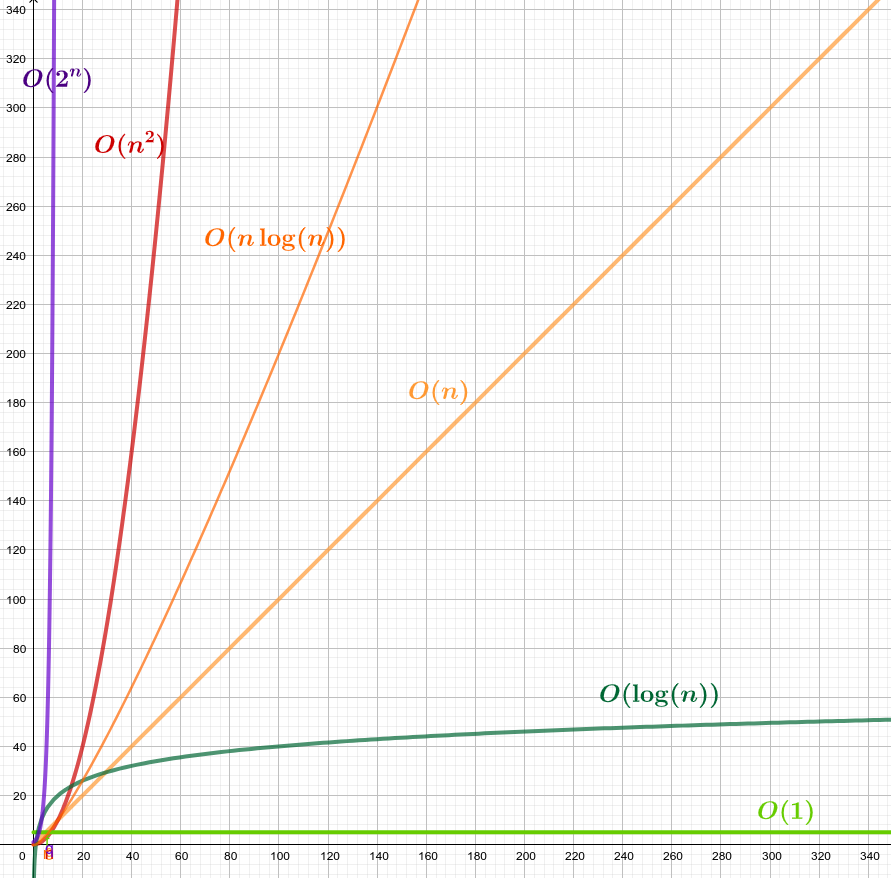
\includegraphics[height=6cm]{complexite.eps}
		\end{center}
	\end{block}
\end{frame}

\begin{frame}[fragile]{\Ctitle}{\stitle}
	\begin{block}{Temps de calcul effectif}
		Sur un ordinateur réalisant 100 million d'opérations par seconde, en notant \textcolor{green}{\faCheck} un temps de calcul quasi instantané et \textcolor{red}{\faTimes} un temps de calcul inaccessible :
		\renewcommand{\arraystretch}{1.4}
		\begin{tabular}{lccccc}
			\cline{2-6}
			\multicolumn{1}{c}{\leavevmode} & \leavevmode$n=10$                                               & $n=100$                                              & $n=1000$                                             & $n=10^6$                                             & $n=10^9$                                         \\
			\hline
			\leavevmode$\GO(\log(n))$        & \textcolor{green}{\faCheck}                          & \textcolor{green}{\faCheck}                          & \textcolor{green}{\faCheck}                          & \textcolor{green}{\faCheck}                          & \textcolor{green}{\faCheck}                      \\
			\hline
			\leavevmode$\GO(n)$              & \leavevmode\onslide<2->{\textcolor{green}{\faCheck}} & \leavevmode\onslide<2->{\textcolor{green}{\faCheck}} & \leavevmode\onslide<2->{\textcolor{green}{\faCheck}} & \leavevmode\onslide<2->{\textcolor{green}{\faCheck}} & \leavevmode\onslide<2->{$\simeq 10$s }           \\
			\hline
			\leavevmode$\GO(n\log(n))$       & \leavevmode\onslide<3->{\textcolor{green}{\faCheck}} & \leavevmode\onslide<3->{\textcolor{green}{\faCheck}} & \leavevmode\onslide<3->{\textcolor{green}{\faCheck}} & \leavevmode\onslide<3->{\textcolor{green}{\faCheck}} & \leavevmode\onslide<3->{$\simeq 1,5$ mn}         \\
			\hline
			\leavevmode$\GO(n^2)$            & \leavevmode\onslide<4->{\textcolor{green}{\faCheck}} & \leavevmode\onslide<4->{\textcolor{green}{\faCheck}} & \leavevmode\onslide<4->{\textcolor{green}{\faCheck}} & \leavevmode\onslide<4->{$\simeq 3$ h }               & \leavevmode\onslide<4->{$\simeq 300$ ans }       \\
			\hline
			\leavevmode$\GO(2^n)$            & \leavevmode\onslide<5->{\textcolor{green}{\faCheck}} & \leavevmode\onslide<5->{\textcolor{red}{\faTimes}}   & \leavevmode\onslide<5->{\textcolor{red}{\faTimes}}   & \leavevmode\onslide<5->\textcolor{red}{\faTimes}     & \leavevmode\onslide<5->\textcolor{red}{\faTimes} \\
			\hline
		\end{tabular}
	\end{block}
\end{frame}

\begin{frame}[fragile]{\Ctitle}{\stitle}
	\begin{exampleblock}{Exemples}
		\begin{itemize}
			\item<1-> On suppose qu'on dispose d'un algorithme de complexité linéaire travaillant sur une liste, il traite une liste de \numprint{1000} éléments en \numprint{0.015} secondes. Donner une estimation du temps de calcul pour une liste de \numprint{250000} éléments.\\
				\onslide<2-> {\textcolor{OliveGreen}{La taille des données a été multiplié par 250, la complexité étant lineaire le temps de calcul sera aussi approximativement multiplié par 250. \\}}
				\onslide<3->{\textcolor{OliveGreen}{$0.015 \times 250 = 3.75$, on peut donc prévoir un temps de calcul d'environ 3,75 secondes}}
			\item<4-> Même question pour un algorithme de complexité quadratique qui traite une liste de \numprint{1000} éléments en \numprint{0.07} secondes.\\
				\onslide<5-> {\textcolor{OliveGreen}{La taille des données a été multiplié par 250, la complexité étant quadratique le temps de calcul sera  approximativement multiplié par $250^2=62500$ \\}}
				\onslide<6->{\textcolor{OliveGreen}{$0.07 \times 62\,500 = 4375$, on peut donc prévoir un temps de calcul d'environ $4\,375$ secondes, c'est-à-dire près d'une heure et 15 minutes !}}
		\end{itemize}
	\end{exampleblock}
\end{frame}

\makess{Complexité des fonctions récursives}
\begin{frame}[fragile]{\Ctitle}{\stitle}
	\begin{block}{Equation de complexité}
		Dans le cas des fonction récursives, la complexité pour une entrée de taille $n$ s'exprime à partir de complexité pour des tailles inférieures. On est donc amené à résoudre une \textit{équation de complexité}.
	\end{block}
	\onslide<2->{
		\begin{exampleblock}{Exemple}
			Par exemple si on considère la version récursive du calcul de la somme d'une liste d'entiers en OCaml :
			\inputpartOCaml{\SPATH/somme.ml}{}{\small}{1}{4}
			Alors on a $C(n) = C(n-1) + a$, et donc $C(n)$ est arithmétique de raison $a$ et $C(n)$ est un $O(n)$.
		\end{exampleblock}}
\end{frame}


\begin{frame}[fragile]{\Ctitle}{\stitle}
	\begin{exampleblock}{Les tours de Hanoï}
		On rappelle que le jeu des tours de Hanoï peut être résolu de façon élégante par récursion. On note $T(n)$ le nombre de mouvement minimal nécessaire afin de résoudre Hanoï avec $n$ disques en utilisant l'algorithme récursif.
		\begin{enumerate}
			\item Déterminer $T(1)$
			\item Exprimer $T(n)$ en fonction $T(n-1)$
			\item En déduire la complexité de l'algorithme.
		\end{enumerate}
	\end{exampleblock}
\end{frame}



\makess{Exemple résolu: recherche dichotomique}
\begin{frame}[fragile]{\Ctitle}{\stitle}
	\begin{exampleblock}{Enoncé : recherche dichotomique}
		On reprend l'exemple de la recherche dichotomique dans un tableau trié:
		\inputpartC{\SPATH/complexite.c}{}{\scriptsize}{12}{26}
		\begin{itemize}
			\item<2-> Prouver que cet algorithme termine
			\item<3-> Prouver qu'il est correct
			\item<4-> Donner sa complexité.
		\end{itemize}
	\end{exampleblock}
\end{frame}

\begin{frame}[fragile]{\Ctitle}{\stitle}
	\begin{exampleblock}{Correction : recherche dichotomique}
		\begin{itemize}
			\item<2->\textcolor{OliveGreen}{Montrons que les valeurs prises par {\tt fin - deb} est un variant de boucle.
				\begin{itemize}
					\item\textcolor{OliveGreen}{{\tt fin-deb} est positif à l'entrée dans la boucle (le tableau est supposé non vide)}
					\item\textcolor{OliveGreen}{{\tt fin-deb} décroît strictement à chaque itération car soit {\tt fin} diminue, soit {\tt }deb augmente}
				\end{itemize}
			}
			\item<3->\textcolor{OliveGreen}{Si la fonction renvoie {\tt true} alors l'élément cherché est bien présent dans le tableau car le test {\tt tab[milieu]==elt} est vraie. Montrons maintenant que si la fonction renvoie {\tt false} alors l'élément n'est pas dans le tableau. Pour cela on montre la propriété suivante : $P$ : \og{} Si {\tt elt} est dans {\tt tab} alors il se trouve entre les indices {\tt deb} et {\tt fin} \fg{}. En effet, :
				\begin{itemize}
					\item<4->\textcolor{OliveGreen}{Cette propriété est vraie à l'entrée dans la boucle puisque {\tt deb=0} et {\tt fin=size-1} la totalité du tableau est couverte.}
					\item<5->\textcolor{OliveGreen}{Cette propriété reste vraie à chaque tour de boucle car puisque le tableau est trié, si {\tt elt} est strictement plus grand que {\tt tab[milieu]} alors il se situe forcément après l'indice {\tt milieu} (et strictement avant dans le cas contraire)}
				\end{itemize}}
		\end{itemize}
	\end{exampleblock}
\end{frame}

\begin{frame}[fragile]{\Ctitle}{\stitle}
	\begin{exampleblock}{Correction : recherche dichotomique}
		\begin{enumerate}
			\item Implémentation itérative :
			      \begin{itemize}
				      \item<2->\textcolor{OliveGreen}{La boucle ne contient que des opérations élémentaires, le coût d'un tour de boucle est donc $O(1)$.}
				      \item<3->\textcolor{OliveGreen}{La taille de l'intervalle de recherche est initialement la taille {\tt n} du tableau et est divisé par deux à chaque itération. Donc le nombre de tours de boucle est un $O(\log(n))$.}
				      \item<4->\textcolor{OliveGreen}{En conclusion, la recherche dichotomique a une complexité logarithmique.}
			      \end{itemize}
			\item<5-> Implémentation récursive :\\
				\textcolor{OliveGreen}{Dans ce cas, on obtient l'équation de complexité $C(n) = C(n/2) + 1$} qui conduit au même résultat.
		\end{enumerate}
	\end{exampleblock}
\end{frame}


\makess{Exemple résolu : tri sélection}
\begin{frame}[fragile]{\Ctitle}{\stitle}
	\begin{exampleblock}{Tri sélection}
		\begin{itemize}
			\item<1-> Rappeler l'algorithme du tri par sélection \\
				\onslide<2->{\textcolor{OliveGreen}{On note $n$ la taille du tableau, pour chaque entier $i=0 \dots n-1$, on échange l'élément situé à l'indice $i$ avec le minimum du tableau depuis l'indice $i$.}}
			\item<3-> Montrer que l'algorithme termine\\
				\onslide<4->{\textcolor{OliveGreen}{L'algorithme ne contient pas de boucle non bornées donc sa terminaison est garantie.}}
			\item<5-> Montrer qu'il est correct
			\item<6-> Déterminer sa complexité
		\end{itemize}
	\end{exampleblock}
\end{frame}


\begin{frame}[fragile]{\Ctitle}{\stitle}
	\begin{exampleblock}{Correction du tri sélection}
		\textcolor{OliveGreen}{Pour montrer que l'algorithme est correct, on prouve  l'invariant : $I$ : \og{}  Les $i$ premiers éléments du tableau sont ceux du tableau trié \fg{}.}
		\begin{itemize}
			\item<2->\textcolor{OliveGreen}{Pour $i=0$, la propriété est vraie (aucun élément n'est encore trié)}
			\item<3->\textcolor{OliveGreen}{En supposant l'invariant vraie au début d'un tour de boucle (c'est-à-dire les $i$ premiers éléments du tableau sont ceux du tableau trié), on montre qu'il est conservé. L'algorithme consiste à placer le minimum des éléments restants à l'indice $i+1$, cet élément est bien celui d'indice $i+1$ dans le tableau trié (il est supérieur aux éléments situés avant et inférieur à ceux qui restent à trier). Et donc l'invariant est conservé.}
		\end{itemize}
	\end{exampleblock}
\end{frame}

\begin{frame}[fragile]{\Ctitle}{\stitle}
	\begin{exampleblock}{Complexité du tri sélection}
		En notant $n$, la taille du tableau
		\begin{itemize}
			\item<1-> Chaque recherche de minimum parcourt au plus la totalité du tableau et est donc un $O(n)$.
			\item<2-> Cette recherche est effectuée $n-1$ fois et est donc aussi un $O(n)$.
			\item<3-> En conclusion la tri par sélection a une complexité en $O(n^2)$.
		\end{itemize}
	\end{exampleblock}
\end{frame}

\makess{Exercice : tri fusion}
\begin{frame}[fragile]{\Ctitle}{\stitle}
	\begin{exampleblock}{Tri fusion}
		\begin{itemize}
			\item<1-> Rappeler le principe de l'algorithme.
			\item<2-> Prouver la terminaison de l'algorithme.
			\item<3-> Montrer qu'il est correct.
			\item<4-> Déterminer sa complexité.
		\end{itemize}
	\end{exampleblock}
\end{frame}



\end{document}